%%%%%%%%%%%%%%%%%%%%%%%%%%%%%%%%%%%%%%%%%%%%%%%%%%%%%%%%%%%%%%%%%%%
%%% Documento LaTeX 																						%%%
%%%%%%%%%%%%%%%%%%%%%%%%%%%%%%%%%%%%%%%%%%%%%%%%%%%%%%%%%%%%%%%%%%%
% Título:		Capítulo 1
% Autor:  	Ignacio Moreno Doblas
% Fecha:  	2014-02-01
% Versión:	0.5.0
%%%%%%%%%%%%%%%%%%%%%%%%%%%%%%%%%%%%%%%%%%%%%%%%%%%%%%%%%%%%%%%%%%%
\chapterbegin{Introducción teórica}
%\minitoc

%\begin{sinopsis}
%\label{sec:chpltx:sinop}
%	
%\end{sinopsis}

\section{Acústica}
\label{sec:RuidoAmb}

\subsection{Nivel de presión sonora}

Definimos como presión acústica o presión sonora el cambio local de presión respecto a la presión atmosférica ambiente (media o en equilibrio) causada por una onda sonora. En el SI, la presión atmosférica (y por ende la acústica) se mide en pascales (Pa), que es igual a una fuerza de un newton (1 N) actuando sobre una superficie de un metro cuadrado ($1 m^2$)

Sin embargo, para mediciones se utiliza el \ac{SPL} definido en~\ref{eq:spl}, una medición logarítmica de la presión sonora efectiva relativa a un nivel de referencia. Por definición:
\begin{equation}
L_p = 10 \log_{10}\left(\frac{{p_\mathrm{rms}}^2}{{p_0}^2}\right) = 20 \log_{10}\left(\frac{p_\mathrm{rms}}{p_0}\right)~\mathrm{dB (SPL)}
\label{eq:spl}
\end{equation}

Donde $p_\mathrm{rms}$ es el valor cuadrático medio de la presion sonora, que es calculado como se muestra en \ref{eq:prms}, medido en $Pa$, y $p_0$ es la presión sonora de referencia, también medida en Pa.

\begin{equation}
p_\mathrm{rms} = \left[ \frac{1}{T} \int_0^T p^2(t)dt \right]^\frac{1}{2}
\label{eq:prms}
\end{equation}

El valor de $p_0$ más comunmente utilizado es $p_0 = 20 \micro Pa (RMS)$, que representa el umbral mínimo de audición humana, y será el utilizado en el presente proyecto.

\subsection{Potencia acústica y densidad espectral de potencia }
Es potencia acústica, o potencia sonora, la medición de la cantidad de energía sonora por unidad de tiempo emitida por una fuente determinada\ref{eq:pa}. Dicha potencia en el \ac{SI} se mide en Watios (W). Dada una fuente sonora, la potencia sonora de dicha fuente es independiente del entorno y de la distancia. La potencia sonora es la potencia total producida por la fuente en todas direcciones. Esto contrasta con la presión sonora, que sí es dependiente de la distancia, ya que es una medición en un punto concreto.

\begin{equation}
P_a = f \cdot v = A \cdot p \cdot u \cdot v
\label{eq:pa}
\end{equation}

Es posible también definir el \ac{SWL}~\ref{eq:swl} de manera análoga al \ac{SPL}, utilizando en este caso una $P_0 = 1 \pico W$. 

\begin{equation}
L_W = 10 \log_{10}\left(\frac{P}{P_0}\right) ~\mathrm{dB (SWL)}
\label{eq:swl}
\end{equation}

\subsubsection{Espectro de frecuencia}
El espectro de frecuencia de una señal en el dominio del tiempo es una representación de dicha señal en el dominio de la frecuencia. El espectro de frecuencia puede ser generado mediante una transformada de Fourier de dicha señal, y los valores resultantes son normalmente amplitud y fase representados en función de la frecuencia.

\subsection{Ruido}
De forma general, es posible definir como ruido cualquier sonido no deseado que interfiera en la recepción de un sonido. El ruido acústico es aquel ruido producido por la mezcla de ondas sonoras de distintas frecuencias y distintas amplitudes. La mezcla se produce a diferentes niveles ya que se conjugan tanto las frecuencias fundamentales como los armónicos que las acompañan.

De las múltiples maneras de clasificar el ruido acústico, son de interés en este proyecto dos:

\subsubsection{Ruido en función de la intensidad y el periodo}

\begin{description}

\item[Ruido fluctuante]
Ruido fluctuante es aquel cuya intensidad no es constante sino que fluctúa a lo largo del tiempo, ya sea de forma periódica o aleatoria.
\item[Ruido impulsivo]
Ruido impulsivo es aquel cuya intensidad aumenta bruscamente durante un impulso. En comparación con el tiempo que transcurre entre un impulso y otro, la duración del impulso es breve.

\end{description}
% division clara
\subsubsection{Ruido en función de la frecuencia}
Existen múltiples modelos de ruido en función de su frecuencia, y la mayoría se implementan en generadores de ruido para ser utilizados en mediciones acústicas. Los principales son:
\begin{description}
\item[Ruido blanco] Quizás el modelo de ruido más conocido, ruido blanco es aquel con la misma cantidad de potencia sonora en cualquier banda de un ancho de banda determinado. Es llamado así por analogía a la luz blanca. Cuando se realiza el diagrama de espectro de un ruido blanco, se observa un espectro plano en frecuencia. Para una señal de audio, es suficiente que esta condición se cumpla en el rango audible, es decir de 20 Hz a 20.000 Hz.
 \begin{figure}[H] \centering
    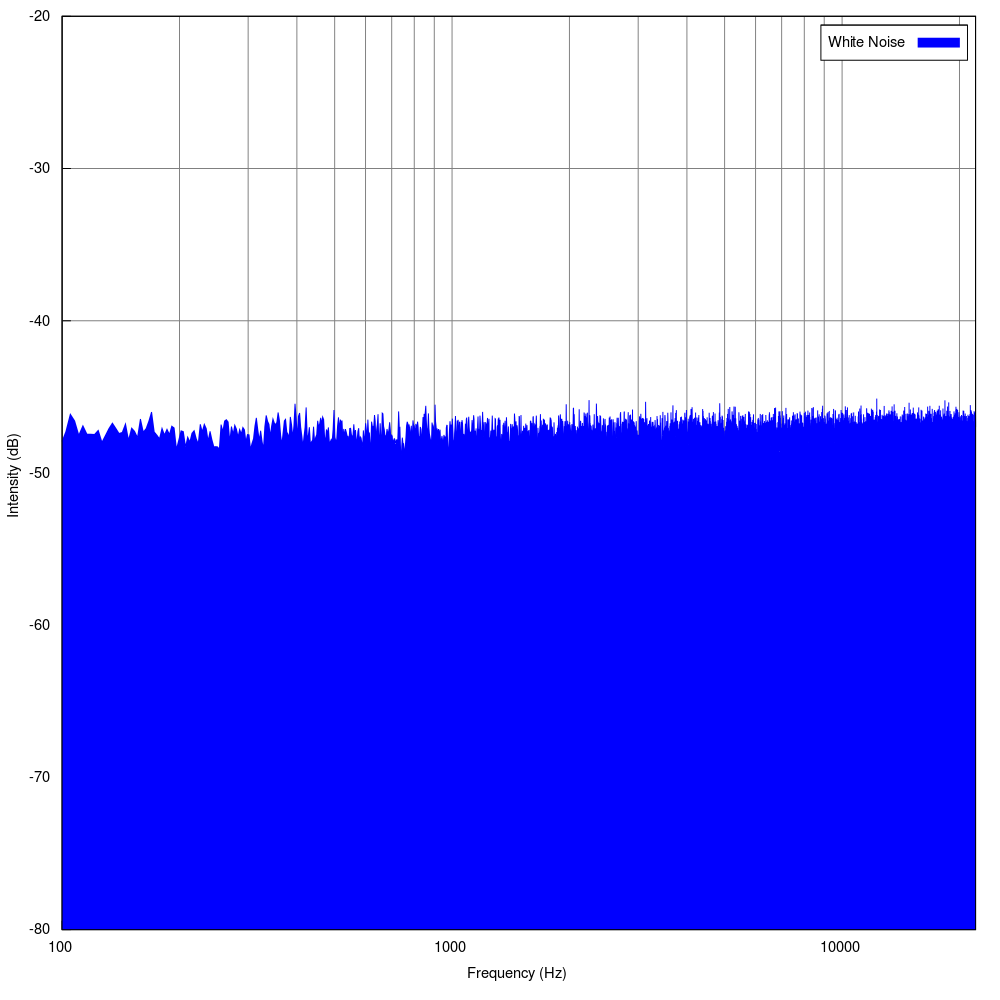
\includegraphics[height=8cm]{graphs/white_noise.png} \caption{Espectro de un ruido blanco}\label{fig:diagrama:ruidoblanco}
\end{figure}
\item[Ruido rosa] El ruido rosa es un ruido con una densidad espectral inversamente proporcional a la frecuencia, de manera que la potencia de ruido de cada octava sea idéntica. Al visualizar su espectro de frecuencia, se aprecia claramente la caída.
 \begin{figure}[H] \centering
    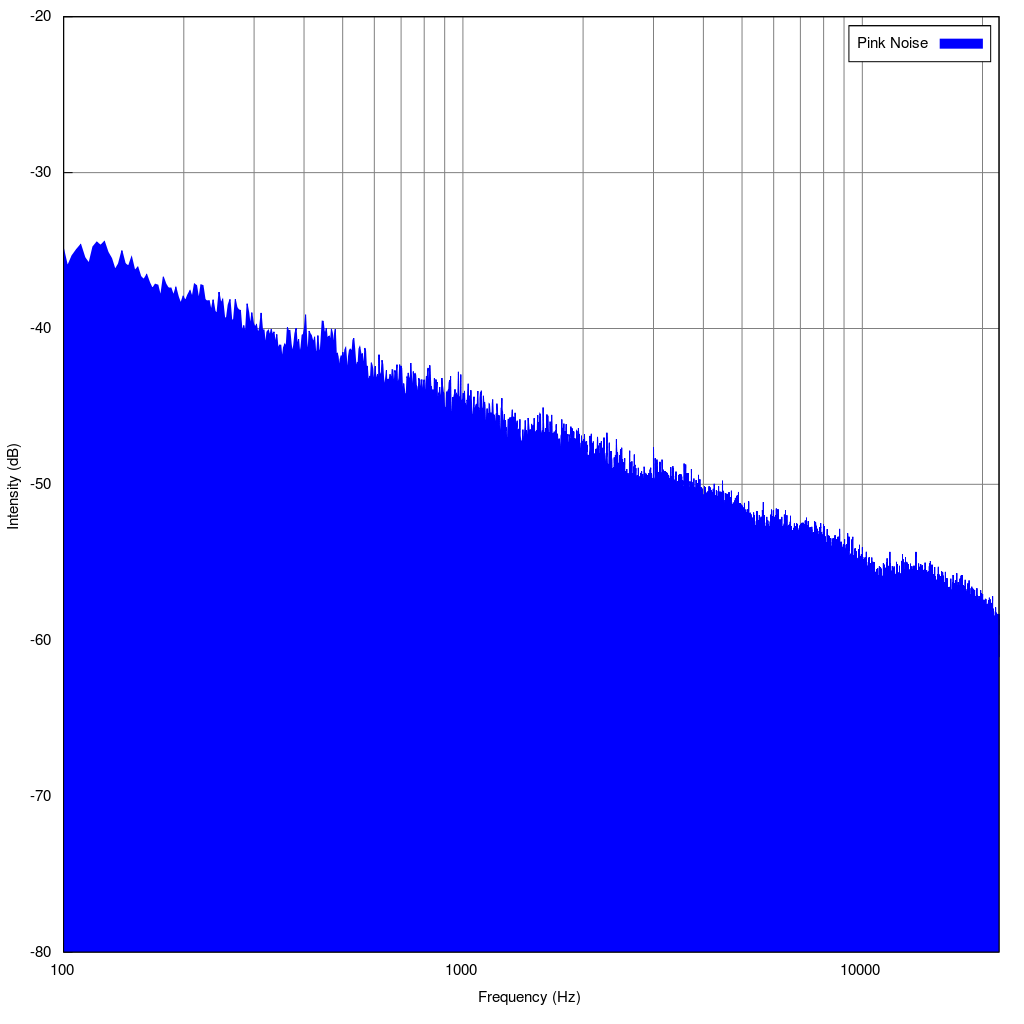
\includegraphics[height=8cm]{graphs/pink_noise.png} \caption{Espectro de un ruido rosa}\label{fig:diagrama:ruidorosa}
\end{figure}

\end{description}

\subsection{Control automático de ganancia (CAG)}
Un \ac{CAG} es un circuito con realimentación cuyo propósito es que la amplitud de la señal a su salida se mantenga controlada a pesar de posibles variaciones de amplitud en la señal de entrada. Dependiendo del diseño del circuito, el nivel medio o de pico es utilizado para ajustar dinámicamente la ganancia del circuito a un valor adecuado.

La vasta mayoría de los fabricantes de teléfonos móviles inteligentes, incorporan semejante función en alguna fase del procesado de la señal de entrada de micrófono, ya sea mediante circuitos analógicos o procesado digital de señal. Es importante tener esto en cuenta, ya que puede ser causa de una aparente compresión de la señal, si se diera el caso. 

\subsection{Modulación por impulsos codificados}

La \ac{PCM}, es un método utilizado para representar digitalmente señales analógicas muestreadas. Es la forma básica de audio digital en ordenadores, discos compactos, telefonía digital y la gran mayoría de aplicaciones de audio digital. En un flujo de audio \ac{PCM}, la amplitud de la señal analógica se muestrea regularmente en intervalos uniformes, y cada muestra se cuantifica al valor más próximo dentro de un rango de posibles valores digitales.

\begin{figure}[H] \centering
    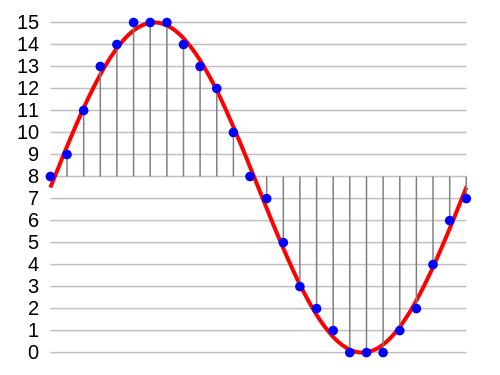
\includegraphics[height=10cm]{graphs/Pcm.png} \caption{Muestreo y cuantización de una señal en PCM de 4 bits}\label{fig:diagrama:PCM}
\end{figure}

Este es el formato en el que el sistema operativo del teléfono inteligente nos proveerá las muestras de audio, y sobre el que trabajaremos.

\section{Android}
\label{sec:AndroidIntro}

Android es un sistema operativo, en sus inicios concebido para dispositivos móviles con pantalla táctil, que ha evolucionado en una plataforma que actualmente también engloba relojes inteligentes, televisores, automóviles e incluso electrodomésticos.

Está basado en el núcleo de Linux, sobre el que corre el entorno de ejecución propio de Android (ya sea Dalvik o ART), y este a su vez ejecuta el código de las aplicaciones, escritas mayoritariamente en Java, aunque se permiten extensiones en C/C++

\begin{figure}[h] \centering
    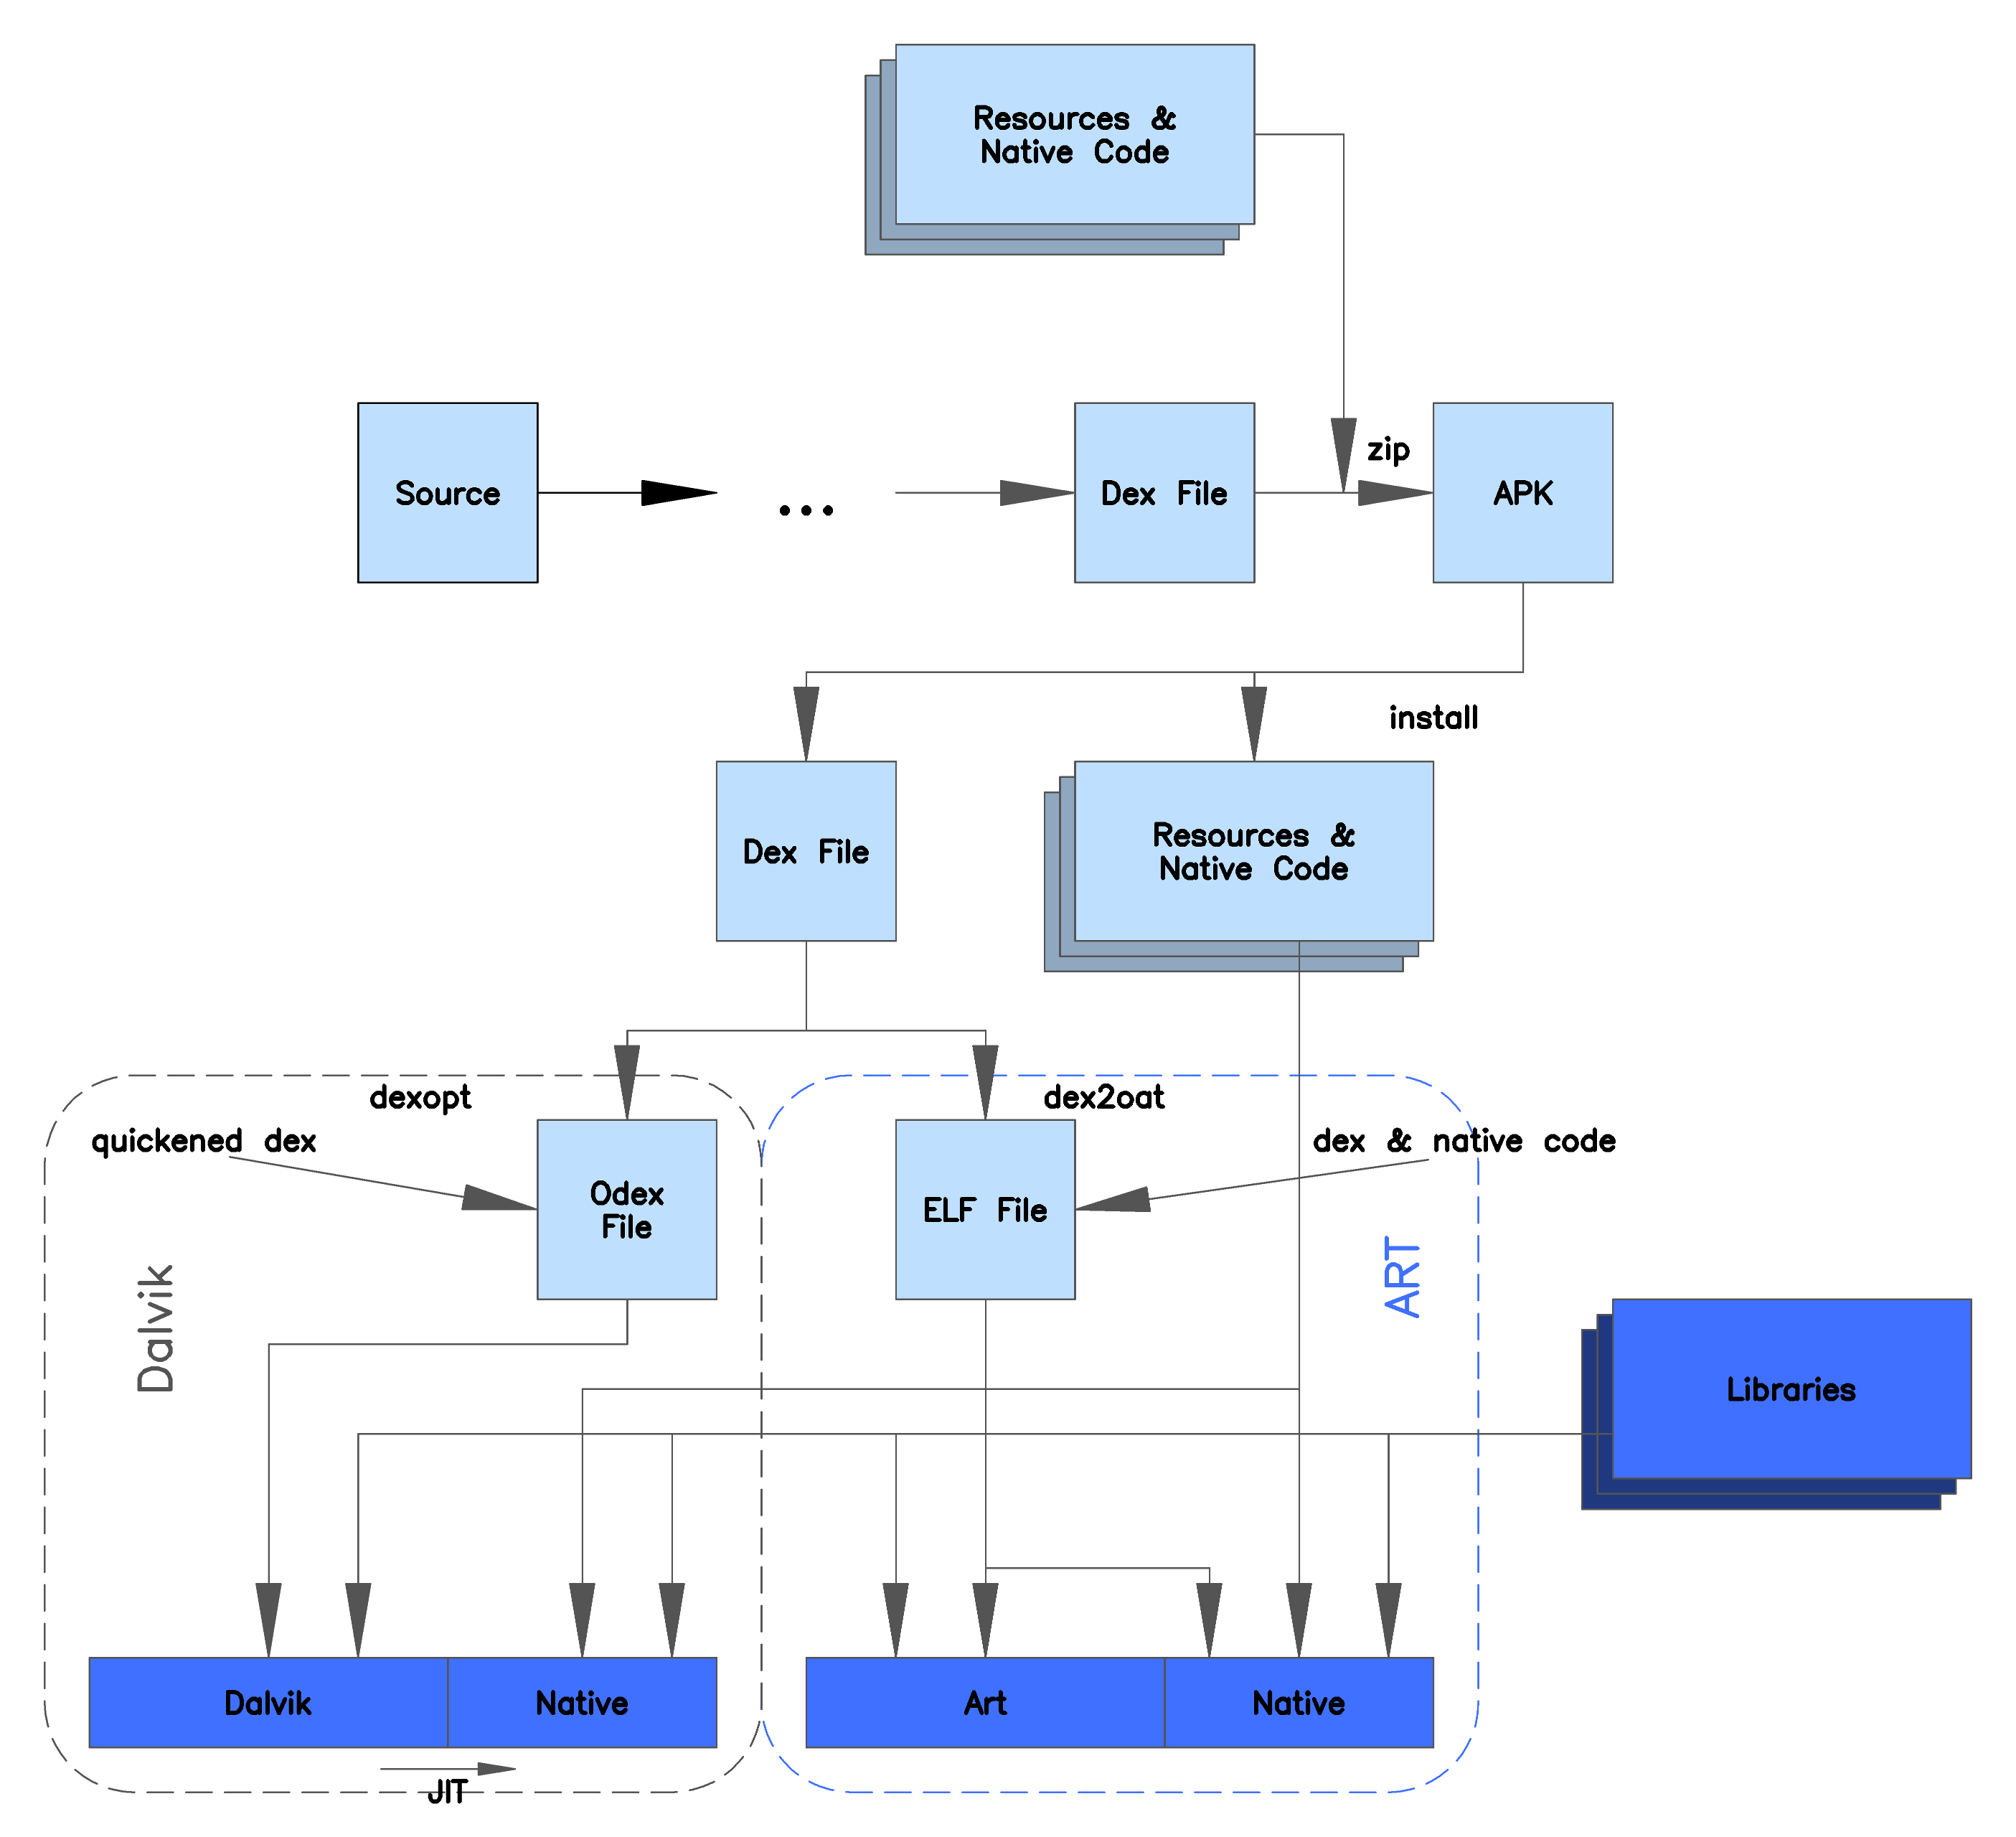
\includegraphics[height=12cm]{graphs/ART_view.png} \caption{Diagrama de la estructura del sistema operativo Android}\label{fig:diagrama:ART}
\end{figure}

\subsection{Interfaz}

La interfaz de usuario por defecto de Android está basada en una manipulación directa, usando entrada táctil con gestos que vagamente corresponden a acciones físicas reales, tales como deslizar, golpear, pellizcar… para manipular objetos en pantalla. Además, la mayoría de dispositivos dispone de un teclado virtual, manipulado de la misma manera. 

La respuesta del sistema a la entrada del usuario está diseñada para ser inmediata y dar una sensación de fluidez, utilizando las capacidades de vibración presentes en la mayoría de los dispositivos para proveer una respuesta háptica (no visual, no auditiva). Adicionalmente, algunas aplicaciones utilizan la información proveída por sensores tales como acelerómetros, giroscopios y sensores de proximidad para responder a interacciones adicionales, como por ejemplo ajustar la orientación de la pantalla cuando el dispositivo se encuentra apaisado o controlar alguna parte de la aplicación basándose en el azimut relativo del dispositivo.

Una parte importante de la interfaz general de Android son las notificaciones, presentes en la barra de estado

\subsection{Componentes de una aplicación}

\subsubsection{Contexto}

Uno de los conceptos más importantes cuando se utiliza la plataforma Android es el contexto, \ttw{Context}. La clase \ttw{Context} en si misma no es más que una interfaz a información global acerca del entorno de una aplicación, y como tal es abstracta. Sin embargo, es importante ser consciente de qué elementos representan un contexto válido y qué elementos no, ya que un contexto permite acceso a recursos y clases específicos de la aplicación, y llamadas al sistema para operaciones a nivel de aplicación, tales como lanzar actividades, emitir mensajes de difusión o recibirlos.

\subsubsection{Actividades}

En android, una actividad (\ttw{Activity}) representa una única cosa concreta que el usuario puede realizar en la aplicación. La mayoría de las actividades interaccionan con el usuario, por tanto la clase \ttw{Activity} se encarga de crear una ventana donde se puedan insertar los componentes de la interfaz de usuario. Aunque las actividades suelen ser vistas por el usuario como ventanas a pantalla completa, también pueden ser usadas en otras múltiples maneras, ya sea como ventanas flotantes, o incrustadas dentro de otra actividad (mediante un \ttw{ActivityGroup})

\subsubsection{Ciclo de vida de una actividad}
Las distintas actividades de las distintas aplicaciones instaladas en el dispositivo Android son gestionadas en forma de una \tit{pila de actividades}.
 
Cuando el sistema Android se inicia, se presenta al usuario una pantalla principal, desde donde puede lanzar varias acciones y aplicaciones. A partir de ahí, cuando una nueva actividad es empezada, se emplaza arriba de la pila y se convierte en la actividad en ejecución. Las actividades previas si las hubiera siempre permanecen por debajo en la pila, y no se traerán al frente hasta que la nueva actividad finalice.

Una actividad tiene cuatro estados básicos:

\begin{description}
    \item[Activa] \hfill \\
     Una actividad está \tit{activa} cuando está presente en primer plano en la pantalla, es decir, arriba de la pila. También se puede decir que la actividad está \tit{En ejecución}.

    \item[Pausada] \hfill \\
    Si una actividad ha perdido el foco (ha dejado de estar en primer plano) pero todavía es visible, es decir, si una nueva actividad que no ocupa la totalidad de la pantalla o es transparente obtiene el primer plano, se encuentra \tit{pausada}. Una actividad pausada se conserva completamente íntegra (mantiene todos los estados y se mantiene suscrita al gestor de ventanas) pero puede ser matada por el sistema en condiciones extremas de baja memoria disponible.

    \item[Parada] \hfill \\
    Si una actividad se encuentra oculta por completo, el sistema la deja \tit{parada}. Mantiene estados e información de los miembros, pero sin embargo al no ser visible por el usuario es más probable que el sistema se deshaga de ella para liberar recursos cuando hagan falta.
    
    \item[Muerta] \hfill \\
    Cuando el sistema decide mover la actividad fuera de memoria, puede o bien finalizarla o matar el proceso. Cuando sea mostrada de nuevo al usuario, debe ser completamente reiniciada y restaurada a su estado previo.
    
\end{description}

\begin{figure}[h] \centering
    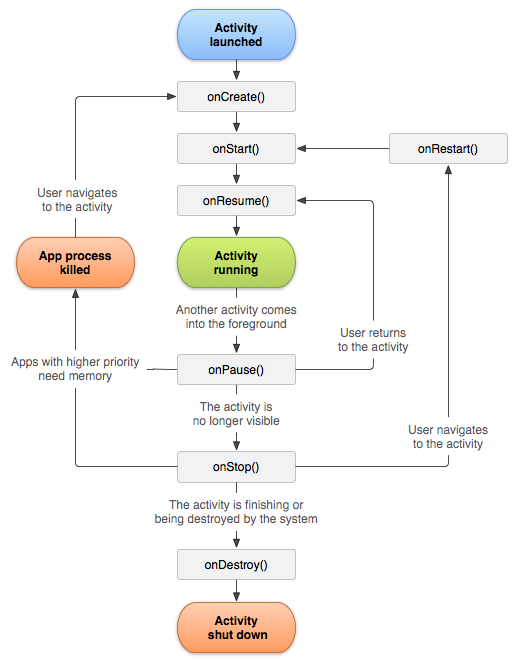
\includegraphics[height=12cm]{graphs/activity_lifecycle.png} \caption{Diagrama del ciclo de vida de una actividad en Android. \cite{androiddevguide}.}\label{fig:diagrama:ActivityLifecycle}
\end{figure}

\subsubsection{Servicios}
\label{ssec:teo:svc}

Un Servicio (\ttw{Service}) es un componente de la aplicación que puede realizar tareas de larga duración en segundo plano y no provee ninguna interfaz de usuario. Otro componente de la aplicación puede iniciar un servicio y este continuará en marcha en segundo plano, incluso si el usuario cambia a otra aplicación distinta. Además, un componente puede adherirse (\ttw{bind}) a un servicio para interacutar con él, e incluso realizar comunicación inter-procesos (IPC por sus siglas en inglés, Inter-Process Communication). Por ejemplo, un servicio puede manejar llamadas de red, reproducir música, realizar operaciones en el sistema de archivos, todo en segundo plano.

Un servicio puede tomar dos estados:

\begin{description}
    \item[Started] \hfill \\
    Un servicio está en estado \ttw{Started} (empezado) cuando un componente de la aplicación, por ejemplo una actividad, lo empieza llamando al método \ttw{startService()}. Una vez empezado de esta manera, un servicio puede continuar en segundo plano de manera indefinida, incluso si el componente que lo empezó ha sido destruído. Normalmente, suelen ser servicios que realizan una única operación y no devuelven ningún resultado. Por ejemplo, puede descargar o subir un archivo en la red. Cuando la operación ha sido completada, el servicio debe pararse a si mismo.
    \item[Bound] \hfill \\
    Un servicio está en estado \ttw{Bound} (adherido) cuando un componente de la aplicación se adhiere a él llamando al método \ttw{bindService()}. Un servicio adherido ofrece una interfaz servidor-cliente que permite a los componentes interaccionar con el servicio, mandar peticiones, obtener resultados, e incluso hacerlo entre distintos procesos mediante comunicación inter-proceso (IPC). Un servicio adherido solamente es activo durante el tiempo que otro componente esté adherido a él. Varios componentes pueden estar adheridos en un momento dado al servicio, pero cuando todos se desadhieren del servicio, el servicio es destruído.

\end{description}

\begin{figure}[h] \centering
    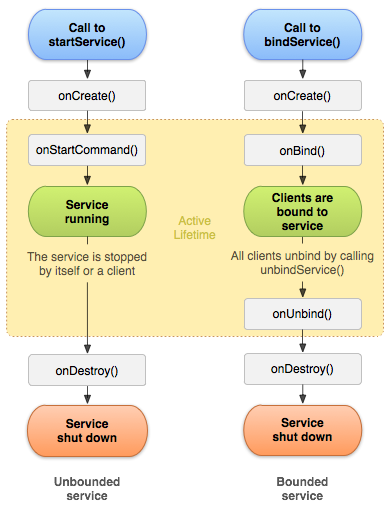
\includegraphics[height=12cm]{graphs/service_lifecycle.png} \caption{Diagrama del ciclo de vida de un servicio.{androiddevguide}}\label{fig:diagrama:ServiceLifecycle}
\end{figure}

Hay que tener cuidado, dado que un servicio corre en el hilo principal de ejecución del proceso que lo llama, a no ser que se especifique lo contrario. Esto implica que, si el servicio va a realizar alguna tarea intensiva en CPU, o alguna operación bloqueante, se debe de crear un nuevo hilo de ejecución dentro del servicio para ese propósito. De no hacerlo, se corre el riesgo de que la aplicación deje de responder y sea matada por el sistema operativo.


\subsection{Vistas}

La interfaz gráfica de usuario en una aplicación Android está construida usando una jerarquía de vistas, objetos de la clase \ttw{View}, y grupos de vistas, objetos de la clase \ttw{ViewGroup}. Los objetos \ttw{View} suelen ser artilugios (widgets) de la interfaz de usuario, tales como botones o campos de texto, y los objetos \ttw{ViewGroup} son contenedores invisibles que definen cómo se posicionan las vistas que dependen de ellos, por ejemplo dispuestas en forma de rejilla o lista vertical.

Android provee un vocabulario XML que se corresponde con las subclases de \ttw{View} y \ttw{ViewGroup}, y permite definir la interfaz de usuario en XML usando una jerarquía de elementos de interfaz de usuario.

\subsection{Procesos e hilos de ejecución}

En sistemas operativos, son básicos los conceptos de proceso e hilo de ejecución. En Android, el sistema operativo comienza un nuevo proceso Linux por cada primer componente de cada aplicación, con un único hilo de ejecución. Por defecto, todos los componentes de la misma aplicación corren en los mismos proceso e hilo de ejecución, el hilo principal de ejecución (\tit{main thread} en inglés). 

En caso de que un componente de una aplicación sea inicializado, y ya exista un proceso para dicha aplicación en el sistema que otro componente de la misma aplicación ha inicializado, el nuevo componente se inicializa dentro del proceso original y usa el mismo hilo de ejecución. Sin embargo, se puede configurar una aplicación de manera que diferentes componentes corran en procesos separados, y siempre se pueden crear hilos de ejecución adicionales para cualquier proceso.

\subsubsection{Procesos}

Como ya ha sido expuesto anteriormente, por defecto todos los componentes de la misma aplicación corren en el mismo proceso, y la mayoría de las aplicacones no deberían de cambiarlo. Sin embargo, es posible controlar qué proceso pertenece a qué componente de ser necesario.

El sistema operativo puede decidir apagar un proceso, cuando la cantidad de memoria disponible sea baja y haya requerimiento de ella por otro proceso que sirva de manera más inmediata al usuario. En este caso, los componentes dentro de dicho proceso que es apagado, son destruidos. Cuando estos componentes sean necesarios de nuevo, un nuevo proceso será comenzado por el sistema operativo para ello.

\subsubsection{Hilos de ejecución}

Previamente se ha mencionado que todos los componentes de la misma aplicación corren en el mismo hilo de ejecución, el hilo principal de ejecución o \tit{main thread}. Este hilo es de suma importancia, dado que carga con la responsabilidad de despachar los eventos al widget de la interfaz de usuario que sea pertinente, incluyendo los eventos de dibujado en pantalla. Es también el hilo de ejecución en el que la aplicación interactúa con los componentes básicos de interfaz de usuario de Android, también conocidos como \tit{Android UI toolkit} (ubicados dentro de los paquetes java \ttw{android.widget} y \ttw{android.view}). Por todo esto, no es extraño encontrar denominado este hilo de ejecución como el hilo de la interfaz de usuario, o \tit{UI Thread}.

Dado que todos los componentes que corren en el mismo porceso son instanciados en el hilo de ejecución principal, las llamadas del sistema operativo a cada componente son despachadas desde dicho hilo. En consecuencia, todos los métodos que responden a retrollamadas del sistema (\tit{system callbacks}), como por ejemplo para indicar que una tecla ha sido pulsada, siempre corren en el hilo principal de ejecución del proceso.

Cuando el usuario toca un botón en la pantalla, el hilo principal de la aplicación despacha el evento de toque al widget pertinente, que reacciona cambiando su estado a presionado y manda una petición de invalidación a la cola de eventos. El hilo de ejecución principal entonces desencola la petición y notifica al widget qque debe de redibujarse.

Cuando una aplicación realiza trabajo intensivo en respuesta a una interacción del usuario, el modelo de hilo de ejecución único puede resultar en una falta de rendimiento. Concretamente, de suceder todo el procesamiento en el hilo principal de ejecución e iniciar tareas de larga ejecución tales como acceso a red o consultas a bases de datos, resultará en un bloqueo completo de la interfaz de usuario y su correspondiente hilo principal. Cuando el hilo de ejecución está bloqueado, no se pueden despachar eventos, eventos de dibujado en pantalla incluidos. Desde el punto de vista del usuario, esto se traduce en una aplicación que parece colgarse. En peores casos, en los que el hilo principal de ejecución está bloqueado por más de unos cuantos segundos (cinco segundos en la actualidad) el sistema operativo entrará en acción y mostrará una pantalla explicando que la aplicación ha dejado de responder, y matará la aplicación bloqueada. 

 Para evitar dicha penalización en el rendimiento, deben usarse hilos de ejecución alternativos para toda tarea que bloquee la ejecución o sea de alta carga procedural.

\subsection{Manejo de archivos}

Para guardar la información recabada en las sesiones de medición realizadas en la aplicación, se usará almacenamiento en archivos de texto plano. Concretamente, se utilizará el formato de valores separados por comas, CSV por sus siglas en inglés. En este formato, como su nombre indica, cada valor de un registro está separdo del contiguo por dicho signo de puntuación. Cada registro está separado de otro por un salto de línea.

La simplicidad que brinda este formato, además de la legibilidad de los archivos al estar estos en texto plano, se presumen adecuados para este proyecto.

\subsection{Ubicación}
\subsubsection{GPS}
El \ac{GPS} es un sistema de navegación por satélite que provee información sobre la posición y el reloj del dispositivo de recepción. El sistema fue desarrollado, instalado y empleado por el Departamento de Defensa de los Estados Unidos. Está constituido por 24 satélites en órbida geosíncrona y se basa en un sistema de triangulación para determinar posiciones con precisión de metros.

El funcionamiento del \ac{GPS} necesita la recepción de la señal de al menos cuatro de los 24 satélites en órbita. En base a dichas señales, que incluyen la identificación del satélite emisor y la hora de reloj de emisión, el aparato receptor sincroniza su reloj interno y calcula el tiempo que tardan en llegar las señales al equipo. Con dicha información, el dispositivo es capaz de conocer su distancia a cada uno de los satélites cuya señal es recibida, y por ende la posición absoluta del punto de medición.

\subsubsection{Servicios Móviles de Google}
Conocer la localización \ac{GPS} del dispositivo móvil es crítico en el funcionamiento de la aplicación. Es posible en un dispositivo Android utilizar el receptor \ac{GPS} a bajo nivel y recibir actualizaciones de posición en formato NMEA. Sin embargo, no se aprovecharían cantidad sustancial de optimizaciones que Google ofrece como parte de \ac{GMS} tales como tiempo de respuesta mejorado, localización mixta y consumo de batería mejorado. 

GMS es un servicio en segundo plano propietario de Google presente en todos los dispositivos Android que satisfagan las condiciones de entrada de la empresa. En este proyecto, la aplicación se conectará a dicho servicio para requerir actualizaciones de posición junto con información extra, por ejemplo la precisión de dicha medida.

\section{Otros}

\subsection{Mapa de calor}
Un mapa de calor es una representación gráfica de datos donde los valores en un plano se representan como colores. Es común utilizarlos superpuestos a otro gráfico o mapa para representar intensidad de una magnitud sobre este. Un ejemplo de mapa de calor se puede apreciar en la figura \ref{fig:saltheatmap}.

\begin{figure}[h] \centering
    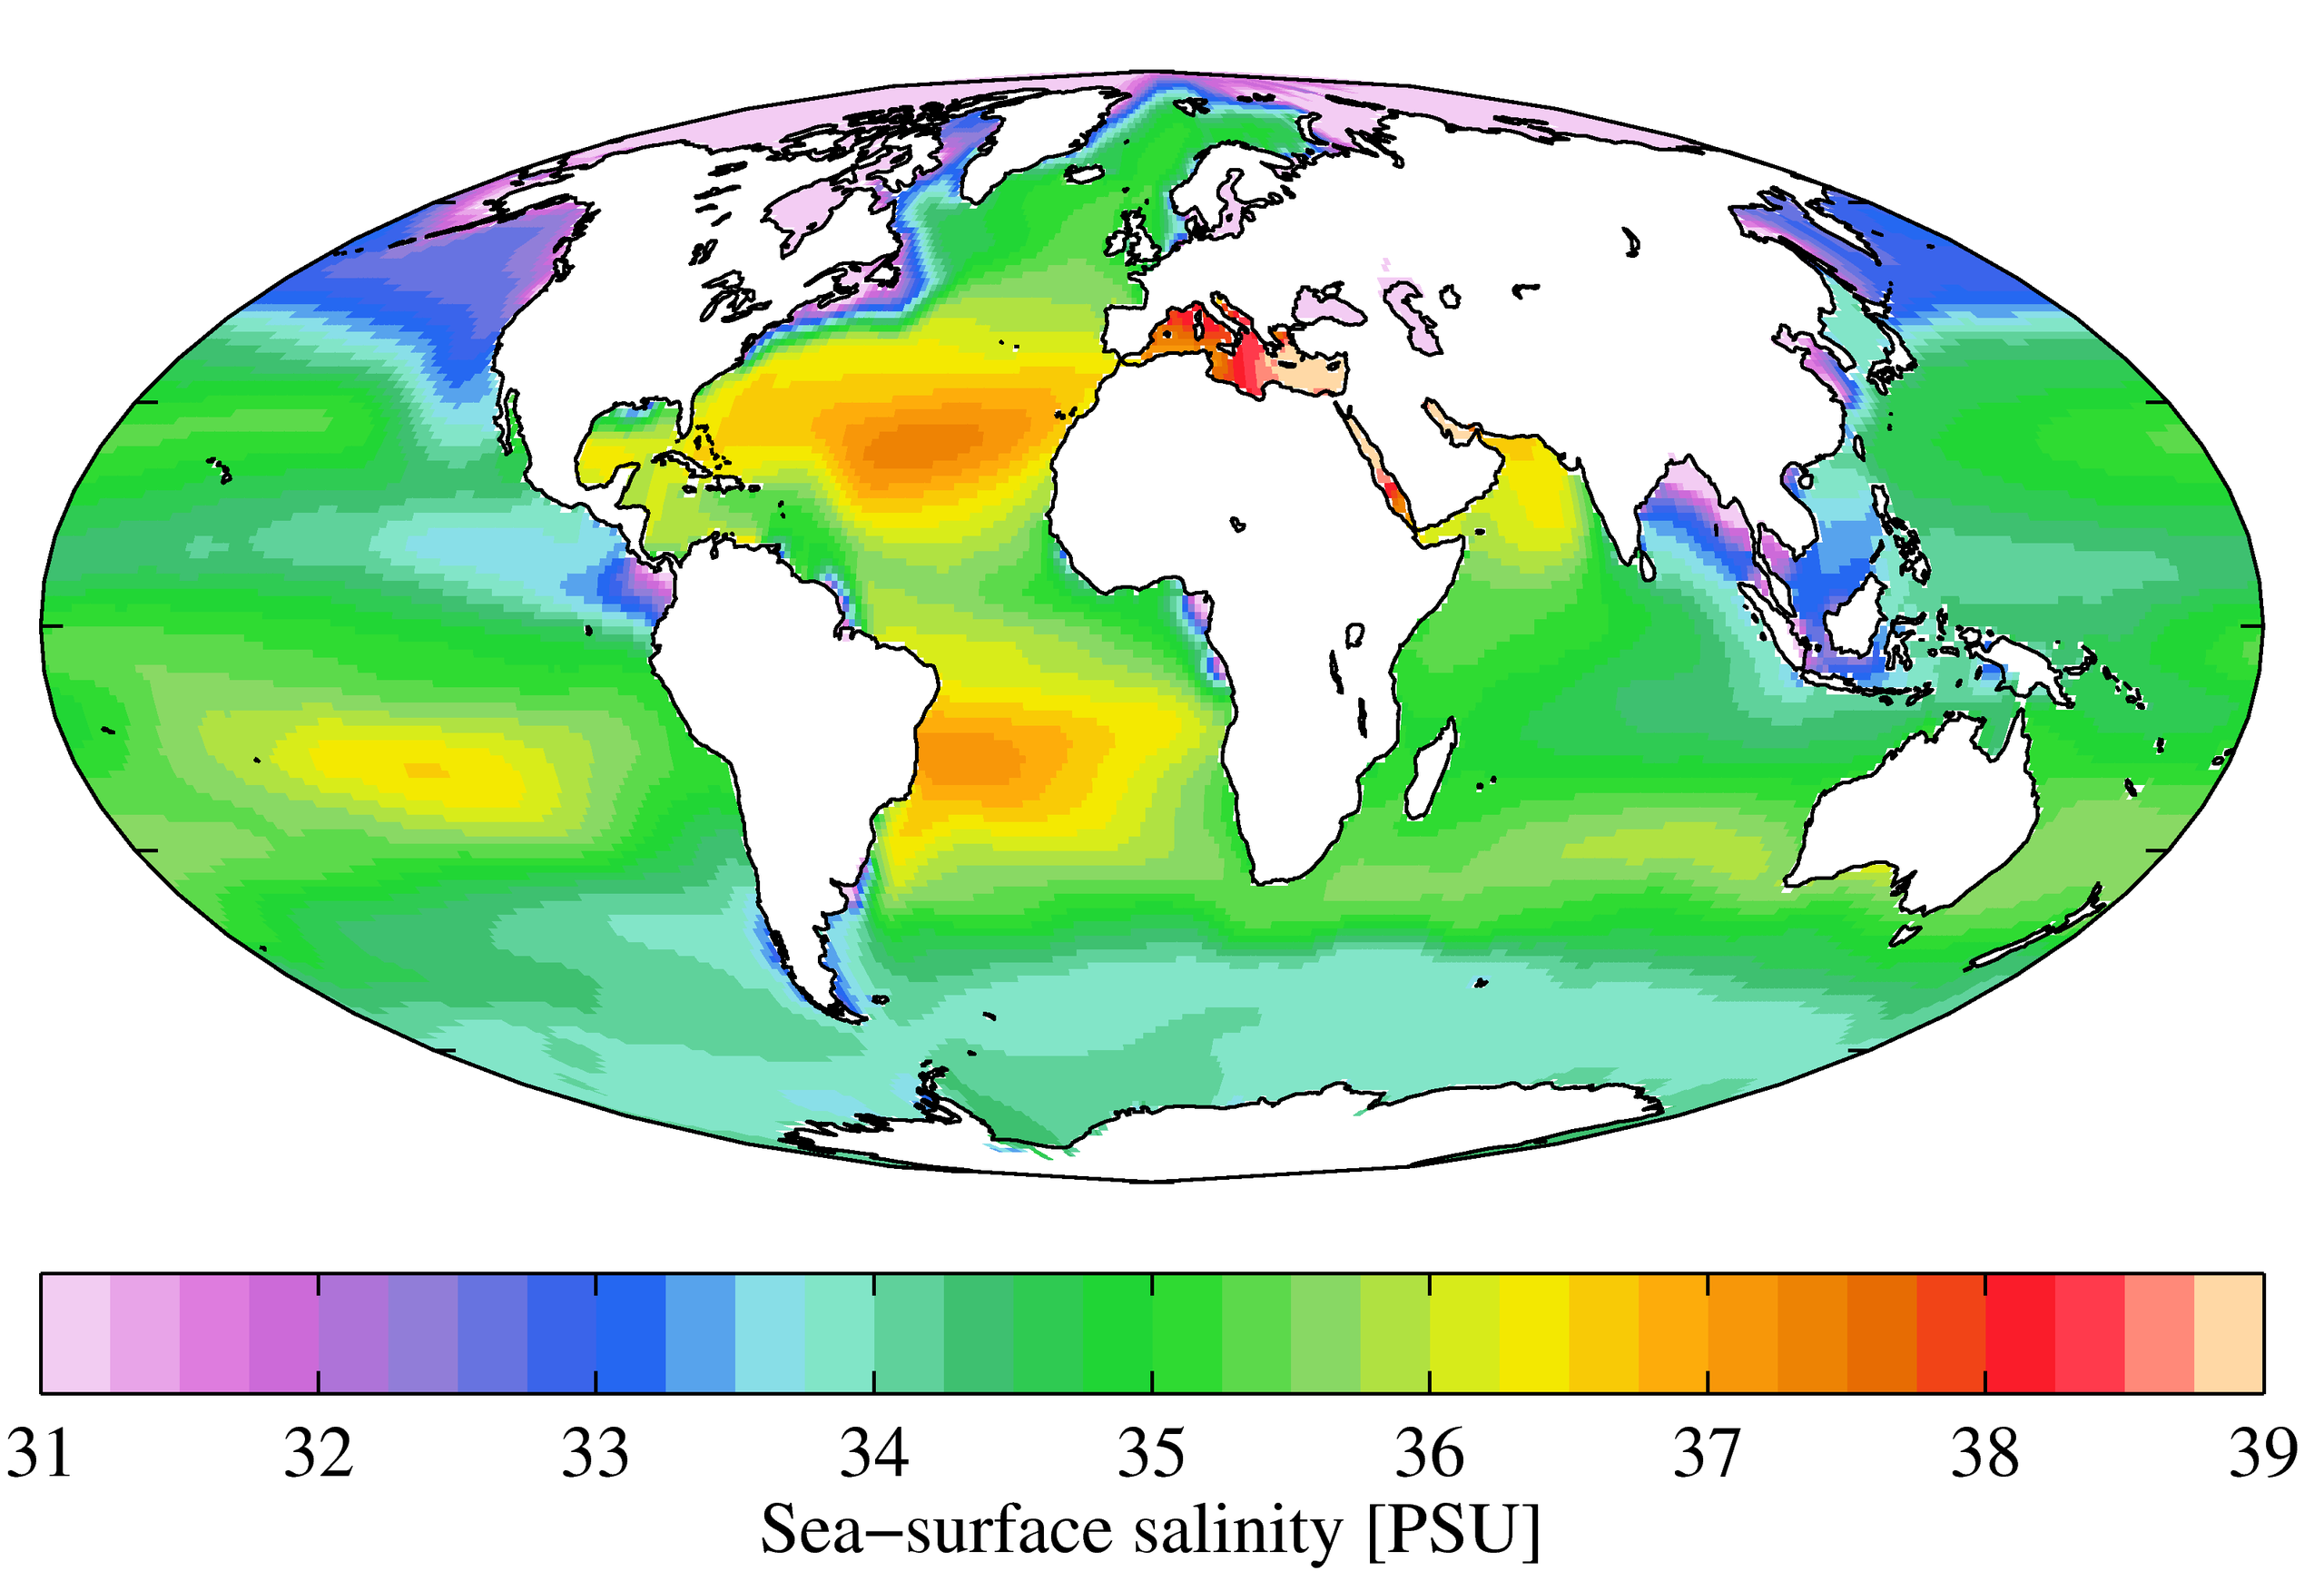
\includegraphics[height=10cm]{graphs/saltheatmap.png}\caption{Mapa de calor mostrando el grado de salinidad de los océanos.\cite{wikiheatmap}}\label{fig:saltheatmap}
\end{figure}



En este proyecto, se utilizarán mapas de calor para representar el nivel de presión sonora registrado en puntos geográficos, de manera que la visualización sea clara y concisa.

\chapterend{}